%
\documentclass[conference,english]{article}

% Some very useful LaTeX packages include:
% (uncomment the ones you want to load)

\usepackage{url} 
\usepackage{listings} 
\usepackage{float}
\usepackage{todonotes}
\usepackage{amsmath}
\usepackage{url}
\usepackage{hyperref}
\usepackage{dirtree}
\usepackage{booktabs}
\usepackage{graphicx}
\usepackage{caption}
\usepackage{subcaption}
\usepackage{fancyvrb}
\usepackage[outdir=./]{epstopdf}
\hypersetup{colorlinks=true,linkcolor=blue}
\makeatletter
\newif\if@restonecol
\makeatother
\let\algorithm\relax
\let\endalgorithm\relax
\usepackage[ruled,vlined]{algorithm2e}
\newcommand{\mytodo}[1]{\textcolor{red}{[#1]}} %for displaying red texts
\renewcommand{\textfraction}{0.01}

\definecolor{cadmiumgreen}{rgb}{0.0, 0.42, 0.24}
\definecolor{auburn}{rgb}{0.43, 0.21, 0.1}

\usepackage{babel,xcolor,framed,marginnote}
\newenvironment{TodoPar}
  {\colorlet{shadecolor}{green!10}\begin{shaded}\marginnote{\fbox{Todo}}}
  {\end{shaded}}
\newenvironment{NotePar}
  {\colorlet{shadecolor}{blue!10}\begin{shaded}\marginnote{\fbox{Note}}}
  {\end{shaded}}
\newenvironment{HypoPar}
  {\colorlet{shadecolor}{red!10}\begin{shaded}\marginnote{\fbox{Hypo}}}
  {\end{shaded}}

\lstdefinelanguage{mybash}{
  tabsize=4,
  language=bash,
  numbers=left,
  frame=tb,
  columns=fullflexible,
  breaklines=true,
  basicstyle=\small\sffamily,
  stringstyle=\small\sffamily\itshape\color{brown}\small,
  commentstyle=\small\sffamily\itshape\color{green}\small,
  backgroundcolor=\color{yellow!20},
  showstringspaces=false,
  showspaces=false,
  mathescape=false,
  classoffset=0,
  keywordstyle=\sffamily\color{blue}\small,
  morekeywords={},
  emph={},
  emphstyle=\linespread{0.85}\color{green}\small,
  linewidth=0.9\linewidth,
  xleftmargin=0.1\linewidth
}

\lstdefinelanguage{myfortran}{%
  tabsize=4,
  language=fortran,
  numbers=left,
  frame=tb,
  columns=fullflexible,
  breaklines=true,
  basicstyle=\small\sffamily,
  stringstyle=\small\sffamily\itshape\color{brown}\small,
  commentstyle=\small\sffamily\itshape\color{green}\small,
  backgroundcolor=\color{yellow!20},
  showstringspaces=false,
  showspaces=false,
  mathescape=false,
  classoffset=0,
  keywordstyle=\sffamily\color{blue}\small,
  morekeywords={},
  emph={},
  emphstyle=\linespread{0.85}\color{green}\small,
  linewidth=0.9\linewidth,
  xleftmargin=0.1\linewidth
}

\lstdefinelanguage{mymatlab}{%
  tabsize=4,
  language=matlab,
  numbers=left,
  frame=tb,
  columns=fullflexible,
  breaklines=true,
  basicstyle=\small\sffamily,
  stringstyle=\small\sffamily\itshape\color{brown}\small,
  commentstyle=\small\sffamily\itshape\color{green}\small,
  backgroundcolor=\color{yellow!20},
  showstringspaces=false,
  showspaces=false,
  mathescape=false,
  classoffset=0,
  keywordstyle=\sffamily\color{blue}\small,
  morekeywords={},
  emph={},
  emphstyle=\linespread{0.85}\color{green}\small,
  linewidth=0.9\linewidth,
  xleftmargin=0.1\linewidth
}

\lstdefinelanguage{mydiff}{
%  tabsize=4,
  frame=tblr,
  breaklines=false,
  basicstyle=\small\sffamily,
  stringstyle=\small\sffamily\itshape\color{brown}\small,
  commentstyle=\small\sffamily\itshape\color{green}\small,
  morecomment=[f][\color{blue}]{@@},     % group identifier
  morecomment=[f][\color{red}]-,         % deleted lines 
  morecomment=[f][\color{cadmiumgreen}]+,       % added lines
  morecomment=[f][\color{magenta}]{---}, % Diff header lines (must appear after +,-)
  morecomment=[f][\color{magenta}]{+++},
  morecomment=[f][\color{auburn}]{!!!},
  backgroundcolor=\color{blue!5},
  linewidth=1.5\linewidth,
  xrightmargin=0.3\linewidth
%  showstringspaces=false,
%  showspaces=false,
%  mathescape=false,
%  classoffset=0,
%  keywordstyle=\sffamily\color{blue}\small,
%  morekeywords={},
%  emph={},
%  emphstyle=\linespread{0.85}\color{green}\small,
}

\lstset{language=myfortran}

% correct bad hyphenation here
\hyphenation{op-tical net-works semi-conduc-tor}
%\renewcommand{\topfraction}{0.99}
\renewcommand{\textfraction}{0.0}
%\renewcommand{\bottomfraction}{0.99}
%\renewcommand{\floatpagefraction}{0.01}
\usepackage{setspace}
\begin{document}


\title{Fortran Testsuite for Automatic Differentiation}
\author{Mahesh Narayanamurthi, Sri Hari Krishna Narayanan, \\ Torsten Bosse and Paul Hovland\\\hfill\\
Mathematics and Computer Science Division\\
Argonne National Laboratory\\
}
\maketitle
\clearpage
\section*{Table of contents}
\tableofcontents
\lstlistoflistings
\clearpage
\section{Abbreviations}
\begin{table}[h]
\centering
\label{abbr_table}
\begin{tabular}{@{}|l|l|@{}}
\hline
\textbf{Abbreviation} & \textbf{Expansion}      \\ \hline
CA           & continuous adjoint \\ \hline
DA           & discrete adjoint \\ \hline
OAD           & openad \\ \hline
TAP          & tapenade \\ \hline
FW           & forward \\ \hline
TL           & tangent linear \\ \hline
ADJ           & adjoint \\ \hline
UD           & undifferentiated \\ \hline
\end{tabular}
\end{table}
\clearpage
\section{Introduction}
\clearpage
\section{Testsuite}
% make the title area
\clearpage
\section{Airfoil}
\subsection{Author and source}
The airfoil test-case is derived from the paper \cite{Giles_2005}. The source code is available \href{http://people.maths.ox.ac.uk/gilesm/codes/airfoil/bangalore05.tar}{here}. The application is a 2D inviscid airfoil code using an unstructured grid. 
\subsection{Description of the mathematical formulation}
For the mathematical formulation refer \cite{Giles_2005}.

\subsection{Directory structure and description of files}
The airfoil test-case is organized into five subdirectories as shown below:\\
\dirtree{%
.1 /. 
.2 air\_foil\_tapenade\DTcomment{Tapenade in Tangent and Adjoint mode}. 
.2 air\_foil\_wopenad\_joint\DTcomment{OpenAD/F in Reverse Joint mode}. 
.2 air\_foil\_wopenad\_split\DTcomment{OpenAD/F in Reverse Split mode}. 
.2 air\_foil\_wopenad\_tanglin\DTcomment{OpenAD/F in Forward mode}. 
.2 mesh\_generator\DTcomment{MATLAB scripts to generate mesh}. 
}
\subsubsection{Differentiated code using Tapenade}
The directory \texttt{air\_foil\_tapenade} contains the files to compile the original \textbf{non-linear flow code}, the \textbf{forward-mode linear flow code} and the \textbf{reverse-mode adjoint flow code}. The binaries (\textbf{files}), corresponding to these, on building the directory are \texttt{airfoil} (\textbf{{airfoil.F}}), \texttt{air\_lin} (\textbf{{air\_lin.F}}) and \texttt{air\_adj} (\textbf{{air\_adj.F}}) respectively. \\

\noindent The binary \texttt{testlinadj} (\textbf{{testlinadj.F}}), which is built along with the rest, constructs a small mesh, initializes flow and tests the linear and adjoint versions of the routines against one another and each of them against the estimate from performing complex finite difference. \\

\noindent The differentiated versions of the original non-linear flow routines are used in the files \texttt{air\_lin.F} and \texttt{air\_adj.F}. These have been obtained by passing the undifferentiated routines to Tapenade on the \href{http://www-tapenade.inria.fr:8080/tapenade/index.jsp}{web}. \\

\noindent The arguments that were used while generating the differentiated version of the routines can be traced back to the Tapenade invocations that are commented in the \texttt{Makefile}, as Tapenade was not available locally at the time. An example of how one would call tapenade to generate the adjoint version \texttt{flux\_face\_bx.f} appears on the following page. 
\clearpage
\begin{lstlisting}[language=mybash]
$ tapenade -backward                                   \
		   -head         flux_face                         \
		   -output       flux_face                         \
		   -vars         "x1 x2 q1 q2 adt1 adt2 res1 res2" \
		   -outvars      "x1 x2 q1 q2 adt1 adt2 res1 res2" \
		   -difffuncname "_bx"                             \
		   routines.f;
\end{lstlisting}
\noindent The listing of files and their descriptions follow.\\
\dirtree{%
.1 /. 
.2 air\_foil\_tapenade.  
.3 adBuffer.c\DTcomment{Tapenade support file}. 
.3 adBuffer.f\DTcomment{Tapenade support file}. 
.3 adBuffer.h\DTcomment{Tapenade support file}. 
.3 adStack.c\DTcomment{Tapenade support file}. 
.3 adStack.h\DTcomment{Tapenade support file}. 
.3 air\_adj.F\DTcomment{Driver for reverse-mode adjoint flow code}. 
.3 airfoil.F\DTcomment{Driver for non-linear flow code}. 
.3 air\_lin.F\DTcomment{Driver for forward-mode linear flow code}. 
.3 flux\_face\_b.f\DTcomment{ADJ version of flux\_face from routines.F}. 
.3 flux\_face\_bx.f\DTcomment{Ditto flux\_face\_b with co-ordinate variations}. 
.3 flux\_face\_d.f\DTcomment{TL version of flux\_face from routines.F}. 
.3 flux\_face\_dx.f\DTcomment{Ditto flux\_face\_d with co-ordinate variations}. 
.3 flux\_wall\_b.f\DTcomment{ADJ version of flux\_wall from routines.F}. 
.3 flux\_wall\_bx.f\DTcomment{Ditto flux\_wall\_b with co-ordinate variations}. 
.3 flux\_wall\_d.f\DTcomment{TL version of flux\_wall from routines.F}. 
.3 flux\_wall\_dx.f\DTcomment{Ditto flux\_wall\_d with co-ordinate variations}. 
.3 input.F\DTcomment{Routines to read and write data}. 
.3 lift\_wall\_b.f\DTcomment{ADJ version of lift\_wall from routines.F}. 
.3 lift\_wall\_bx.f\DTcomment{Ditto lift\_wall\_b with co-ordinate variations}. 
.3 lift\_wall\_d.f\DTcomment{TL version of lift\_wall from routines.F}. 
.3 lift\_wall\_dx.f\DTcomment{Ditto lift\_wall\_d with co-ordinate variations}. 
.3 print\_active.F\DTcomment{Routines to record matrices and vectors}. 
.3 routines.F\DTcomment{Real and complex versions of non-linear routines}. 
.3 testlinadj.F\DTcomment{Derivatives test code}. 
.3 time\_cell\_b.f\DTcomment{ADJ version of time\_cell from routines.F}. 
.3 time\_cell\_bx.f\DTcomment{Ditto time\_cell\_b with co-ordinate variations}. 
.3 time\_cell\_d.f\DTcomment{TL version of time\_cell from routines.F}. 
.3 time\_cell\_dx.f\DTcomment{Ditto time\_cell\_d with co-ordinate variations}. 
.3 const.inc\DTcomment{Constants common block}. 
.3 flow.dat\DTcomment{Initial flow - scaled up problem size}. 
.3 flow.dat.bak\DTcomment{Initial flow - original}. 
.3 grid.dat\DTcomment{Unstructured grid - scaled up problem size}. 
.3 grid.dat.bak\DTcomment{Unstructured grid - original}. 
.3 Makefile\DTcomment{Build commands}. 
}
\clearpage
\subsubsection{Differentiated code using OpenAD in Reverse Joint Mode}
For details on reverse joint mode refer \cite{Griewank_2008} and \cite{Utke_2014}.\\

\noindent The directory \texttt{air\_foil\_wopenad\_joint} contains the files to compile the original \textbf{non-linear flow code} and the \textbf{reverse-mode adjoint flow code}. The binaries (\textbf{files}), corresponding to these, on building the directory are \texttt{airfoil} (\textbf{{airfoil.F}}) and \texttt{air\_adj} (\textbf{{air\_adj.F}}) respectively. \\

\begin{TodoPar}\noindent The binary \texttt{testlinadj} (\textbf{{testlinadj.F}}), which was earlier used to validate the forward-linear and reverse-adjoint routines in the \texttt{air\_foil\_tapenade} subdirectory, is not yet available to test OpenAD/F as modifications have to be done to use \texttt{oad\_active} type in the source code.\end{TodoPar}

\noindent The adjoint version of the original non-linear flow routines are used in the file  \texttt{air\_adj.F}. These have been obtained by passing the undifferentiated routines to OpenAD/F in reverse-joint mode.\\

\noindent For details on how to call OpenAD/F in reverse-joint mode refer \cite{Utke_2014}. The listing of files and their descriptions follow.\\

\dirtree{%
.1 /. 
.2 air\_foil\_wopenad\_joint.  
.3 adStack.c.bak\DTcomment{Unused Tapenade support file}. 
.3 air\_adj.F\DTcomment{Driver for reverse-mode adjoint flow code}. 
.3 airfoil.F\DTcomment{Driver for non-linear flow code}. 
.3 air\_lin.F.bak\DTcomment{Unused forward-mode linear flow code driver}. 
.3 const.inc\DTcomment{Constants common block}. 
.3 flow.dat\DTcomment{Initial flow - scaled up problem size}. 
.3 flow.dat.bak\DTcomment{Initial flow - original}. 
.3 flux\_face.F\DTcomment{UD version of flux\_face from routines.F}. 
.3 flux\_wall.F\DTcomment{UD version of flux\_wall from routines.F}. 
.3 grid.dat\DTcomment{Unstructured grid - scaled up problem size}. 
.3 grid.dat.bak\DTcomment{Unstructured grid - original}. 
.3 iaddr.c\DTcomment{OpenAD/F support file}. 
.3 input.F\DTcomment{Routines to read and write data}. 
.3 lift\_wall.F\DTcomment{UD version of lift\_wall from routines.F}. 
.3 Makefile\DTcomment{Build commands}. 
.3 Makefile.bak\DTcomment{Unused makefile}. 
.3 print\_active.F\DTcomment{Routines to record matrices and vectors}. 
.3 routines.F\DTcomment{Real and complex versions of non-linear routines}. 
.3 testlinadj.F.bak\DTcomment{Unused derivatives test code}. 
.3 time\_cell.F\DTcomment{UD version of time\_cell from routines.F}.  
}

\clearpage
\subsubsection{Differentiated code using OpenAD in Reverse Split Mode}
For details on reverse split mode refer \cite{Griewank_2008} and \cite{Utke_2014}.\\

\noindent The directory \texttt{air\_foil\_wopenad\_split} contains the files to compile the original \textbf{non-linear flow code} and the \textbf{reverse-mode adjoint flow code}. The binaries (\textbf{files}), corresponding to these, on building the directory are \texttt{airfoil} (\textbf{{airfoil.F}}) and \texttt{air\_adj} (\textbf{{air\_adj.F}}) respectively. \\

\begin{TodoPar}\noindent The binary \texttt{testlinadj} (\textbf{{testlinadj.F}}), which was earlier used to validate the forward-linear and reverse-adjoint routines in the \texttt{air\_foil\_tapenade} subdirectory, is not yet available to test OpenAD/F as modifications have to be done to use \texttt{oad\_active} type in the source code.\end{TodoPar}

\noindent The adjoint version of the original non-linear flow routines are used in the file  \texttt{air\_adj.F}. These have been obtained by passing the undifferentiated routines to OpenAD/F in reverse-split mode.\\

\noindent For details on how to call OpenAD/F in reverse-split mode refer \cite{Utke_2014}. The listing of files and their descriptions follow.\\

\dirtree{%
.1 /. 
.2 air\_foil\_wopenad\_split.  
.3 adStack.c.bak\DTcomment{Unused Tapenade support file}. 
.3 air\_adj.F\DTcomment{Driver for reverse-mode adjoint flow code}. 
.3 airfoil.F\DTcomment{Driver for non-linear flow code}. 
.3 air\_lin.F.bak\DTcomment{Unused forward-mode linear flow code driver}. 
.3 const.inc\DTcomment{Constants common block}. 
.3 flow.dat\DTcomment{Initial flow - scaled up problem size}. 
.3 flow.dat.bak\DTcomment{Initial flow - original}. 
.3 flux\_face.F\DTcomment{UD version of flux\_face from routines.F}. 
.3 flux\_wall.F\DTcomment{UD version of flux\_wall from routines.F}. 
.3 grid.dat\DTcomment{Unstructured grid - scaled up problem size}. 
.3 grid.dat.bak\DTcomment{Unstructured grid - original}. 
.3 iaddr.c\DTcomment{OpenAD/F support file}. 
.3 input.F\DTcomment{Routines to read and write data}. 
.3 lift\_wall.F\DTcomment{UD version of lift\_wall from routines.F}. 
.3 Makefile\DTcomment{Build commands}. 
.3 Makefile.bak\DTcomment{Unused makefile}. 
.3 print\_active.F\DTcomment{Routines to record matrices and vectors}. 
.3 routines.F\DTcomment{Real and complex versions of non-linear routines}. 
.3 testlinadj.F.bak\DTcomment{Unused derivatives test code}. 
.3 time\_cell.F\DTcomment{UD version of time\_cell from routines.F}.  
}

\clearpage
\subsubsection{Differentiated code using OpenAD in Forward Mode}
\noindent The directory \texttt{air\_foil\_wopenad\_tanglin} contains the files to compile the original \textbf{non-linear flow code} and the \textbf{forward-mode linear flow code}. The binaries (\textbf{files}), corresponding to these, on building the directory are \texttt{airfoil} (\textbf{{airfoil.F}}) and \texttt{air\_lin} (\textbf{{air\_lin.F}}) respectively. \\

\begin{TodoPar}\noindent The binary \texttt{testlinadj} (\textbf{{testlinadj.F}}), which was earlier used to validate the forward-linear and reverse-adjoint routines in the \texttt{air\_foil\_tapenade} subdirectory, is not yet available to test OpenAD/F as modifications have to be done to use \texttt{oad\_active} type in the source code.\end{TodoPar}

\noindent The tangent-linear version of the original non-linear flow routines are used in the file  \texttt{air\_lin.F}. These have been obtained by passing the undifferentiated routines to OpenAD/F in forward mode.\\

\noindent For details on how to call OpenAD/F in forward-mode refer \cite{Utke_2014}. The listing of files and their descriptions follow.\\

\dirtree{%
.1 /. 
.2 air\_foil\_wopenad\_tanglin.  
.3 airfoil.F\DTcomment{Driver for non-linear flow code}. 
.3 air\_lin.F\DTcomment{Driver for forward-mode linear flow code driver}. 
.3 const.inc\DTcomment{Constants common block}. 
.3 flow.dat\DTcomment{Initial flow - scaled up problem size}. 
.3 flow.dat.bak\DTcomment{Initial flow - original}. 
.3 flux\_face.F\DTcomment{UD version of flux\_face from routines.F}. 
.3 flux\_wall.F\DTcomment{UD version of flux\_wall from routines.F}. 
.3 grid.dat\DTcomment{Unstructured grid - scaled up problem size}. 
.3 grid.dat.bak\DTcomment{Unstructured grid - original}. 
.3 iaddr.c\DTcomment{OpenAD/F support file}. 
.3 input.F\DTcomment{Routines to read and write data}. 
.3 lift\_wall.F\DTcomment{UD version of lift\_wall from routines.F}. 
.3 Makefile\DTcomment{Build commands}. 
.3 Makefile.bak\DTcomment{Unused makefile}. 
.3 print\_active.F\DTcomment{Routines to record matrices and vectors}. 
.3 routines.F\DTcomment{Real and complex versions of non-linear routines}. 
.3 testlinadj.F.bak\DTcomment{Unused derivatives test code}. 
.3 time\_cell.F\DTcomment{UD version of time\_cell from routines.F}. 
}
\clearpage
\subsubsection{Mesh generation}\label{mesh_gen}
The directory \texttt{mesh\_generator} packs a MATLAB script \texttt{naca0012.m} which can be used to generate larger meshes. The \texttt{airfoil} example can read the meshes that are in the ``old'' format. This can be specified while calling the script from MATLAB like below.
\hfill\break
\begin{lstlisting}[language=mymatlab, numbers=none]
>> naca0012(`old')
\end{lstlisting}
The script generates a \texttt{grid.dat} file where the first row contains the number of nodes, cells and edges in the mesh and the corresponding mesh data follows. The size of the mesh can be controlled by changing the parameters \texttt{I} and \texttt{J} in the MATLAB script.

\begin{NotePar}
\noindent To use a new grid file in airfoil code, the parameters \texttt{maxnode}, \texttt{maxcell} and \texttt{maxedge} have to be set appropriately in each of the driver files. Also, note that the \texttt{maxcell} is one more than corresponding value from the \texttt{grid.dat} file.
\end{NotePar}
\subsection{Modifications performed}
Refer section \ref{diff_airfoil}
\subsection{How to build}
Running make as below, in each of the four subdirectories beginning with ``airfoil'' will build the  binaries \texttt{airfoil}, \texttt{air\_lin} and \texttt{air\_adj}.
\hfill\break
\begin{lstlisting}[language=mybash, numbers=none]
    $ make
\end{lstlisting}
\begin{NotePar}
\noindent  The directories \texttt{air\_foil\_wopenad\_split} and \texttt{air\_foil\_wopenad\_joint} will only build the binaries \texttt{airfoil} and \texttt{air\_adj}.\\

\noindent Likewise the directory \texttt{air\_foil\_wopenad\_tanglin} will only build the binaries \texttt{airfoil} and \texttt{air\_lin}.
\end{NotePar}
\subsection{How to verify}
At the time of writing, there exists no script that can validate the output from any of the binaries. All versions of the binary \texttt{airfoil} should produce exactly the same output.\\

\noindent Validation by eyeballing the output from each version of the binaries \texttt{air\_lin} and  \texttt{air\_adj} has been performed. It is of significance to note that the outputs from \texttt{air\_lin} and  \texttt{air\_adj} should also be within certain fixed tolerance from one another.

\begin{TodoPar}
\noindent It will be valuable to write a \texttt{python} script that will take as input two \texttt{csv} files and find the \texttt{max-norm} of the difference between the corresponding entries. Other norms may also be computed. 
\end{TodoPar}

\noindent In order to test the derivatives, since the code does computations deterministically i.e. there are no convergence related iterations, each version of \texttt{airfoil} can be made to write the computed derivatives to a file and the files themselves can be passed to the \texttt{python} script.\\

\begin{TodoPar}
\noindent Additionally, the binary \texttt{testlinadj} can be used to test linear and adjoint routines in \texttt{air\_foil\_tapenade} directory. And by modifying \texttt{testlinadj.F} suitably - by making use of \texttt{oad\_active} type - in each of the other directories, validation can be performed.
\end{TodoPar}
\subsection{How to extend}
\subsubsection{Generating larger grids and flows}
Section \ref{mesh_gen} discusses how to create a larger mesh. Once a larger mesh has been created, corresponding flow has to be now generated. The \texttt{airfoil} application provides all the necessary code to do this. \\

\noindent The file \texttt{input.F} has a section of code that goes as below.\\

\begin{lstlisting}[language=myfortran]
c
c------ read in data from flow file, initialising if necessary
c
        open(1,file='flow.dat',status='old')
        read(1,*) p, r, mach, alpha
        alpha = alpha*datan(1.0d0)/45.0d0
        p = 1.0d0
        r = 1.0d0
        u = dsqrt(gam*p/r)*mach
        e = p/(r*gm1) + 0.5d0*u**2
c
        do ic = 1, ncell
          q(1,ic) = r
          q(2,ic) = r*u
          q(3,ic) = 0.d0
          q(4,ic) = r*e
        enddo
c
        do ic = 1, ncell
          read(1,*,err=999,end=999) (q(ipde,ic),ipde=1,4)
        enddo
 999    close(1)
\end{lstlisting}
\hfill \break
In order to generate the corresponding flows, lines \texttt{19-22} of \texttt{input.F} may be initially commented. A base flow is initialized in lines \texttt{12-17}. Using this, the binary \texttt{airfoil} may be executed for a long time period. When the binary finishes executing, it writes the solution at the end of the simulation to \texttt{flow.dat} file. This file may later be used by uncommenting the lines \texttt{19-22} of \texttt{input.F} to warm-start the simulation with a hopefully converged flow.\\

\noindent Paraphrasing an email from one of the authors of \cite{Giles_2005}:

\begin{verbatim}
 The airfoil testcase was developed several years ago for an
 an AD project using Tapenade:
 http://people.maths.ox.ac.uk/~gilesm/codes/airfoil/index.html

 The input.F file initializes a uniform flow at a given 
 pressure, density, mach number and angle of attack. For 
 this technique (of initializing the flow) to be used with
 larger meshes, the timestep in the CFD calculations may
 need to be  lowered to handle strong initial transients.

 The authors used to run the simulation using just this
 technique, letting the simulation warm up by running 
 several iterations. At the end of each simulation the
 updated flow is written to the same flow.dat file which
 can later be used to continue the simulation, if needed.
\end{verbatim}
\subsubsection{Throwing more stuff on the tape, artificially}
One of the intended uses of this airfoil test-case is to test checkpointing algorithms in AD tools. With regards to \texttt{OpenAD/F}\clearpage 
\section{Power Generation (not Power Grid)}
\subsection{Author and source}
The power generation test-case is derived from the summer project \cite{Rao_2013} at ANL. A copy of the source code, with some minor bug fixes to the original, is included in the \texttt{git} repository as described below. The application is an optimal control problem to `\textit{`maximize the input power to a generator while limiting its mechanical angle oscillation}'' as described in the reference above.
\subsection{Description of the mathematical formulation}\label{power_cont_adj_math}
A general framework for an \textcolor{red}{optimal control} \cite{Sandu_2012} problem is given below:
\[ \theta \,=\, \text{argmin} \;\; \Psi(x, \theta) = \int_{t_0}^{t_F} r\big(x(t), \theta\big)\, dt \,+\, w\big(x(t_F), \theta\big)\]
\[ \text{subject to:} \;\; x' = f(t, x, \theta), \; t_0 \leq t \leq t_F, \; x(t_0) = x_0(\theta) \]
Here, we seek to minimize the cost function $\Psi$ by choosing $\theta$. However, noting that the parameter $\theta$ also decides the value of $x(t_F)$ on which the cost function is dependent. This dependency relation of $x(t_F)$ on $\theta$ comes from the constraint ODE.\\

\noindent Using continuous adjoints, the gradient of the \textcolor{red}{hamiltonian} with respect to the parameters $\theta$ can be written as:

\[\nabla_{\theta} \Psi = w_{\theta}^T\big(x(t_F), \theta\big) + \bigg(\frac{d x_0}{d \theta}\bigg)^T \,.\, \lambda(t_0) +\;\int_{t_0}^{t_F} \bigg(f_{\theta}^T(t, x, \theta) \,.\, \lambda(t) + r_{\theta}^T\big(x,\theta\big)\bigg) dt\]

\noindent The actual problem that is being solved by the power generation example is given below:

\[ p_m \,=\, \text{argmin} \;\; \Psi( p_m, \phi) = - p_m \,+\, c \int_{t_0}^{t_F} \big((\phi - \phi_S)_{+}\big)^4 \, dt\]
subject to: 
\begin{eqnarray*}
\frac{d\phi}{dt} &=& \omega_B (\omega - \omega_S)\\
\frac{d\omega}{dt} &=& \frac{\omega_S}{2H} (p_m - p_{max} sin(\phi) - D(\omega - \omega_S)),\; t_0 \leq t \leq t_F \\
\phi(t_0) &=& sin^{-1}\bigg(\frac{p_m}{p_{max}}\bigg) \\
\omega(t_0) &=& 1 
\end{eqnarray*}
$\omega$: frequency, \, $\phi$: phase angle,\, $p_m$: parameter\\

\noindent The \texttt{MATLAB} code uses continuous adjoints to compute the gradient of the cost function $\Psi$ with respect to the parameter $p_m$.
\clearpage
\subsection{Directory structure and description of files}
The power generation test-case is organized into five subdirectories as shown below:\\
\dirtree{%
.1 /. 
.2 MATLAB\DTcomment{Original MATLAB files with minor bug fixes}. 
.2 Fortran/ContinuousAdj\DTcomment{\texttt{Fortran} port with continuous adjoints}. 
.2 Fortran/DiscreteAdj/OpenAD/TangLin\DTcomment{\texttt{OpenAD/F} in FW Mode}. 
.2 Fortran/DiscreteAdj/OpenAD/Joint\DTcomment{\texttt{OpenAD/F} in RJ Mode}. 
.2 Fortran/DiscreteAdj/OpenAD/Split\DTcomment{\texttt{OpenAD/F} in RS Mode}. 
.2 Fortran/DiscreteAdj/Tapenade\DTcomment{Tapenade in Adjoint Mode}.  
}
\subsubsection{\texttt{MATLAB} version}
The directory \texttt{MATLAB} contains the original files with some minor bug fixes to comply with \cite{Rao_2013} and \cite{Sandu_2012}. The \texttt{MATLAB} version of the code uses the continuous adjoint formulation as mentioned in the earlier references.\\

\noindent The listing of files and their descriptions follow.\\
\dirtree{%
.1 /. 
.2 MATLAB.  
.3 main.m\DTcomment{Driver file for the power generation model}. 
.3 sens\_check.m\DTcomment{Model with continuous adjoint}. 
.3 TSOPF\_Experiments.pdf\DTcomment{Same as \cite{Rao_2013}}. 
}
\hfill\break
\noindent The \texttt{MATLAB} version can be executed like below.\\

\begin{lstlisting}[language=mymatlab, numbers=none]
>> main
\end{lstlisting}
\hfill \break
\noindent The plots generated by the \texttt{MATLAB} version appear on the following page.
\clearpage
\begin{figure}[h]
\centering
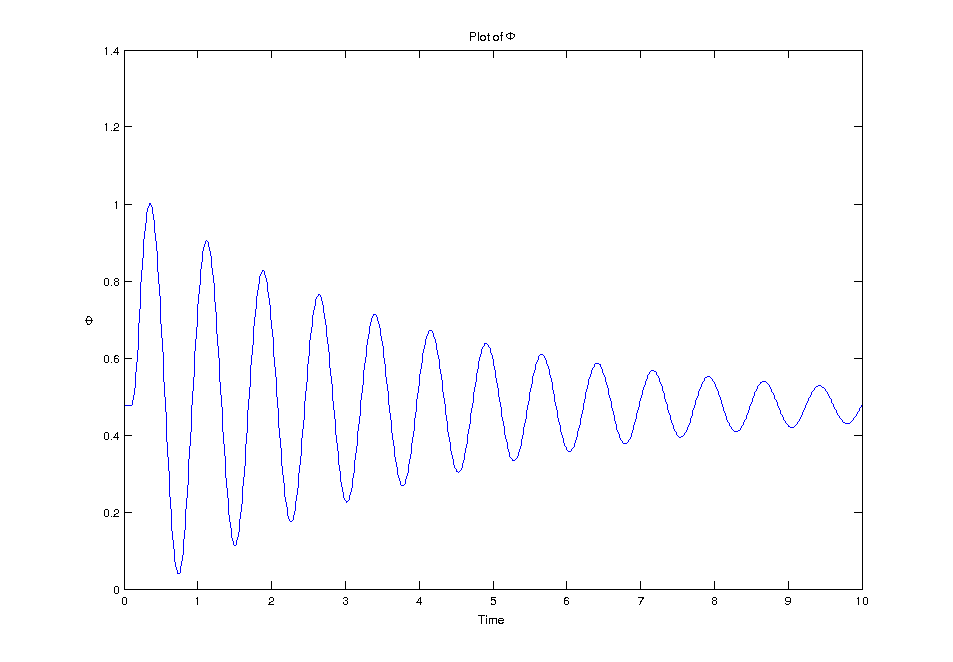
\includegraphics[width=1.2\linewidth]{../Code/miniApps/power_grid/phi_matlab.png}
\label{fig:plot_of_phi_matlab}
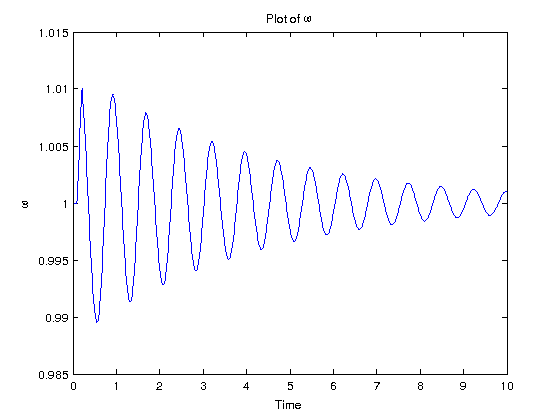
\includegraphics[width=1.2\linewidth]{../Code/miniApps/power_grid/omega_matlab.png}
\label{fig:plot_of_omega_matlab}
\end{figure}
\clearpage
\subsubsection{\texttt{Fortran} port with continuous adjoints}\label{sec_fortran_port_power}
The directory \texttt{Fortran/ContinousAdj} contains the port of the \texttt{MATLAB} version. L-BFGS \cite{Byrd_1996},\cite{Zhu_1997},\cite{Morales_2011} was used to perform the optimization in the \texttt{Fortran} port, a copy of which can be obtained \href{http://users.iems.northwestern.edu/~nocedal/lbfgsb.html}{here}.\\

\noindent The directory \texttt{Fortran/ContinousAdj} contains the files to compile continous adjoint version of the optimal control problem listed in \ref{power_cont_adj_math} and \cite{Rao_2013}. The binaries (\textbf{files}), corresponding to these, on building the directory are \texttt{powergrid} (\textbf{{main.f90}}).\\

\noindent The listing of files and their descriptions follow.\\

\dirtree{%
.1 /. 
.2 Fortran/ContinuousAdj.  
.3 blas.f\DTcomment{L-BFGS support file}. 
.3 constants.f90\DTcomment{Constants and shared variables}. 
.3 gnufor2.f90\DTcomment{\texttt{Fortran} bindings for GNUPlot}. 
.3 iterate.dat\DTcomment{Output from L-BFGS optimization routine}. 
.3 lbfgsb.f\DTcomment{L-BFGS optimization routine}. 
.3 linpack.f\DTcomment{L-BFGS support file}. 
.3 main.f90\DTcomment{Driver for the continuous adjoint port}. 
.3 Makefile\DTcomment{Build commands}. 
.3 print\_active.f\DTcomment{Routines to pretty print matrices and vectors}. 
.3 timer.f\DTcomment{L-BFGS support file}. 
}
\hfill \break
\noindent The plots generated by the \texttt{Fortran} version using continuous adjoints appear on the following page.
\clearpage
\begin{figure}[h]
\centering
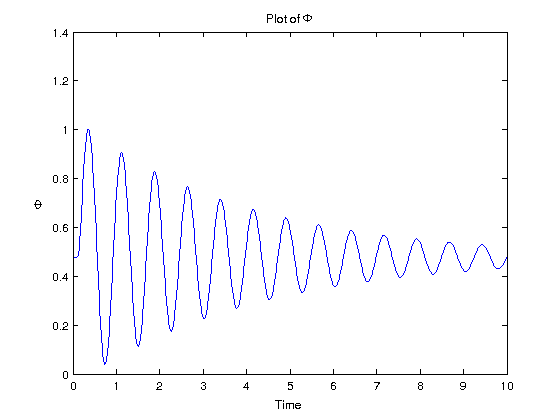
\includegraphics[width=1.2\linewidth]{../Code/miniApps/power_grid/phi_fortran_ca.png}
\label{fig:plot_of_phi_fortran_ca}
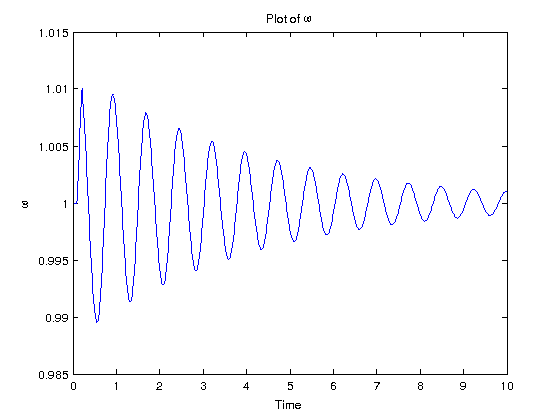
\includegraphics[width=1.2\linewidth]{../Code/miniApps/power_grid/omega_fortran_ca.png}
\label{fig:plot_of_omega_fortran_ca}
\end{figure}
\clearpage
\subsubsection{\texttt{Fortran} port with \texttt{OpenAD/F} in Reverse Split Mode}
For details on reverse split mode refer \cite{Griewank_2008} and \cite{Utke_2014}.\\

\noindent The directory \texttt{Fortran/DiscreteAdj/OpenAD/Split} contains the files to compile the discrete adjoint version of the \texttt{Fortran} port in section \ref{sec_fortran_port_power}. L-BFGS \cite{Byrd_1996},\cite{Zhu_1997},\cite{Morales_2011} was used to perform the optimization in the discrete adjoint version of the Fortran port, a copy of which can be obtained \href{http://users.iems.northwestern.edu/~nocedal/lbfgsb.html}{here}.\\

\noindent The binaries (\textbf{files}), corresponding to these, on building the directory are \texttt{powergrid} (\textbf{{main.f90}}).\\

\noindent The adjoint version of the forward model is used in the file  \texttt{main.f90}. These have been obtained by passing the undifferentiated routines to \texttt{OpenAD/F} in reverse-split mode.\\

\noindent For details on how to call \texttt{OpenAD/F} in reverse-split mode refer \cite{Utke_2014}. The listing of files and their descriptions follow.\\

\dirtree{%
.1 /. 
.2 Fortran/DiscreteAdj/OpenAD/Split.  
.3 blas.f\DTcomment{L-BFGS support file}. 
.3 constants.f90\DTcomment{Constants and shared variables}. 
.3 gnufor2.f90\DTcomment{\texttt{Fortran} bindings for GNUPlot}. 
.3 iterate.dat\DTcomment{Output from L-BFGS optimization routine}. 
.3 lbfgsb.f\DTcomment{L-BFGS optimization routine}. 
.3 linpack.f\DTcomment{L-BFGS support file}. 
.3 main.f90\DTcomment{Driver for the discrete adjoint of port}. 
.3 Makefile\DTcomment{Build commands}. 
.3 Makefile\_continuous\_adjoint\DTcomment{Build commands for CA model}. 
.3 numerics.f90\DTcomment{FW and ADJ model routines from \texttt{main.f90}}. 
.3 print\_active.f\DTcomment{Routines to pretty print matrices and vectors}. 
.3 timer.f\DTcomment{L-BFGS support file}.  
}

\hfill \break
\noindent The plots generated by the \texttt{Fortran} version using discrete adjoints generated by \texttt{OpenAD/F} in reverse-split mode appear on the following page.

\clearpage
\begin{figure}[h]
\centering
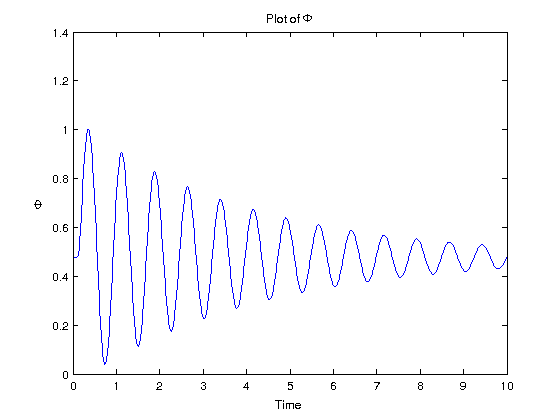
\includegraphics[width=1.2\linewidth]{../Code/miniApps/power_grid/phi_fortran_da_oad_rs.png}
\label{fig:phi_fortran_da_oad_rs}
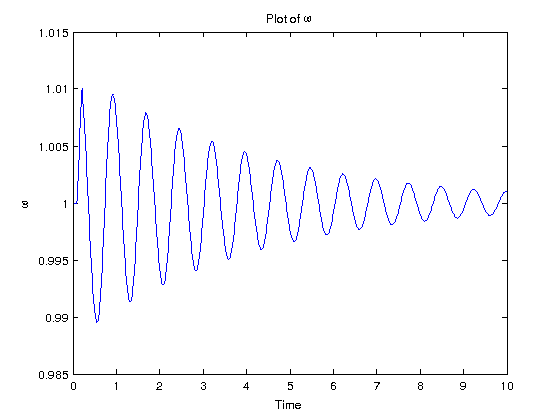
\includegraphics[width=1.2\linewidth]{../Code/miniApps/power_grid/omega_fortran_da_oad_rs.png}
\label{fig:omega_fortran_da_oad_rs}
\end{figure}
\clearpage
\subsubsection{\texttt{Fortran} port with \texttt{OpenAD/F} in Reverse Joint Mode}
For details on reverse joint mode refer \cite{Griewank_2008} and \cite{Utke_2014}.\\

\noindent The directory \texttt{Fortran/DiscreteAdj/OpenAD/Joint} contains the files to compile the discrete adjoint version of the \texttt{Fortran} port in section \ref{sec_fortran_port_power}. L-BFGS \cite{Byrd_1996},\cite{Zhu_1997},\cite{Morales_2011} was used to perform the optimization in the discrete adjoint version of the Fortran port, a copy of which can be obtained \href{http://users.iems.northwestern.edu/~nocedal/lbfgsb.html}{here}.\\

\noindent The binaries (\textbf{files}), corresponding to these, on building the directory are \texttt{powergrid} (\textbf{{main.f90}}).\\

\noindent The adjoint version of the forward model is used in the file  \texttt{main.f90}. These have been obtained by passing the undifferentiated routines to \texttt{OpenAD/F} in reverse-joint mode.\\

\noindent For details on how to call \texttt{OpenAD/F} in reverse-joint mode refer \cite{Utke_2014}. The listing of files and their descriptions follow.\\

\dirtree{%
.1 /. 
.2 Fortran/DiscreteAdj/OpenAD/Joint.  
.3 blas.f\DTcomment{L-BFGS support file}. 
.3 constants.f90\DTcomment{Constants and shared variables}. 
.3 gnufor2.f90\DTcomment{\texttt{Fortran} bindings for GNUPlot}. 
.3 iterate.dat\DTcomment{Output from L-BFGS optimization routine}. 
.3 lbfgsb.f\DTcomment{L-BFGS optimization routine}. 
.3 linpack.f\DTcomment{L-BFGS support file}. 
.3 main.f90\DTcomment{Driver for the discrete adjoint of port}. 
.3 Makefile\DTcomment{Build commands}. 
.3 Makefile\_continuous\_adjoint\DTcomment{Build commands for CA model}. 
.3 numerics.f90\DTcomment{FW and ADJ model routines from \texttt{main.f90}}. 
.3 print\_active.f\DTcomment{Routines to pretty print matrices and vectors}. 
.3 timer.f\DTcomment{L-BFGS support file}.  
}

\hfill \break
\noindent The plots generated by the \texttt{Fortran} version using discrete adjoints generated by \texttt{OpenAD/F} in reverse-joint mode appear on the following page.

\clearpage
\begin{figure}[h]
\centering
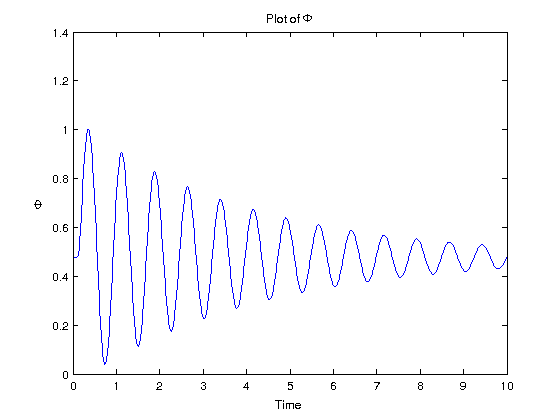
\includegraphics[width=1.2\linewidth]{../Code/miniApps/power_grid/phi_fortran_da_oad_rj.png}
\label{fig:phi_fortran_da_oad_rj}
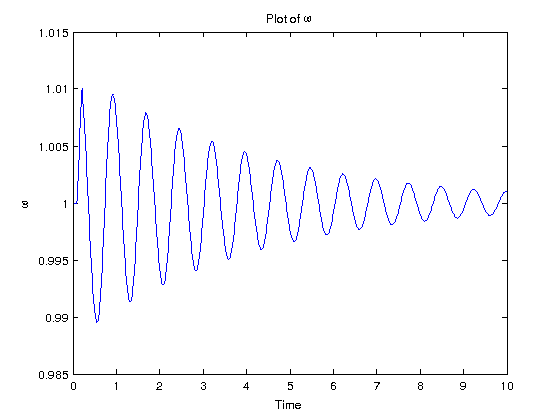
\includegraphics[width=1.2\linewidth]{../Code/miniApps/power_grid/omega_fortran_da_oad_rj.png}
\label{fig:omega_fortran_da_oad_rj}
\end{figure}
\clearpage
\subsubsection{\texttt{Fortran} port with \texttt{OpenAD/F} in Forward Mode}
\noindent The directory \texttt{Fortran/DiscreteAdj/OpenAD/TangLin} contains the files to compile the forward-mode linear version of the \texttt{Fortran} port in section \ref{sec_fortran_port_power}. L-BFGS \cite{Byrd_1996},\cite{Zhu_1997},\cite{Morales_2011} was used to perform the optimization in the discrete adjoint version of the Fortran port, a copy of which can be obtained \href{http://users.iems.northwestern.edu/~nocedal/lbfgsb.html}{here}.\\

\noindent The binaries (\textbf{files}), corresponding to these, on building the directory are \texttt{powergrid} (\textbf{{main.f90}}).\\

\noindent The tangent linear version of the forward model is used in the file  \texttt{main.f90}. These have been obtained by passing the undifferentiated routines to \texttt{OpenAD/F} in forward mode.\\

\noindent For details on how to call \texttt{OpenAD/F} in forward mode refer \cite{Utke_2014}. The listing of files and their descriptions follow.\\

\dirtree{%
.1 /. 
.2 Fortran/DiscreteAdj/OpenAD/Joint.  
.3 blas.f\DTcomment{L-BFGS support file}. 
.3 constants.f90\DTcomment{Constants and shared variables}. 
.3 gnufor2.f90\DTcomment{\texttt{Fortran} bindings for GNUPlot}. 
.3 iterate.dat\DTcomment{Output from L-BFGS optimization routine}. 
.3 lbfgsb.f\DTcomment{L-BFGS optimization routine}. 
.3 linpack.f\DTcomment{L-BFGS support file}. 
.3 main.f90\DTcomment{Driver for the discrete adjoint of port}. 
.3 Makefile\DTcomment{Build commands}. 
.3 Makefile\_continuous\_adjoint\DTcomment{Build commands for CA model}. 
.3 numerics.f90\DTcomment{FW and ADJ model routines from \texttt{main.f90}}. 
.3 print\_active.f\DTcomment{Routines to pretty print matrices and vectors}. 
.3 timer.f\DTcomment{L-BFGS support file}.  
}

\begin{TodoPar}
\noindent Unfortunately, at the time of writing, the tangent-linear version of the forward model does not converge resulting in completely corrupted results. Further the code exhibits a strange behavior, in that it gives yet another completely different result when a single print statement is added after passing it through \texttt{OpenAD/F}. 
\end{TodoPar}

\noindent Quoting verbatim an excerpt of an email that I had written about this behavior (on the following page):
\clearpage
\begin{Verbatim}[xleftmargin=2em]
The numerical routines are all in numerics.f90. 
When I was debugging I noticed that the 
non-linear solve inside Crank Nicolson 
scheme was not converging properly. There is a 
quantity called conv_err which is the convergence 
error. There is an if block which checks whether
the convergence error has fallen below a 
threshold : 1e-8 before moving onto the next time
point in the integrator. 

I was trying to print conv_err (after passing 
through open ad) before the if block. I ensured
that the openad command was disables in the 
makefile. But adding this print changes the 
output when run in comparison to without the
print statement.

The process is as follows:

1) Run Make
2) open the generated numerics.pre....post.f90
3) Add the print statement before the if block 
which check conv_err < 1e-8 inside Crank Nicolson 
scheme
4) Open Makefile
5) Comment out `openad` call
6) Make
7) Run powergrid (result different from without 
adding the print statement in step 3)

The source code is under 
/Code/miniApps/powergrid/DiscreteAdj/OpenAD/TangLin
\end{Verbatim}
\clearpage
\subsection{Modifications performed}
Refer section \ref{diff_airfoil}
\subsection{How to build}
Running make as below, in each of the four subdirectories beginning with ``airfoil'' will build the  binaries \texttt{airfoil}, \texttt{air\_lin} and \texttt{air\_adj}.
\hfill\break
\begin{lstlisting}[language=mybash, numbers=none]
    $ make
\end{lstlisting}
\begin{NotePar}
\noindent  The directories \texttt{air\_foil\_wopenad\_split} and \texttt{air\_foil\_wopenad\_joint} will only build the binaries \texttt{airfoil} and \texttt{air\_adj}.\\

\noindent Likewise the directory \texttt{air\_foil\_wopenad\_tanglin} will only build the binaries \texttt{airfoil} and \texttt{air\_lin}.
\end{NotePar}
\subsection{How to verify}
At the time of writing, there exists no script that can validate the output from any of the binaries. All versions of the binary \texttt{airfoil} should produce exactly the same output.\\

\noindent Validation by eyeballing the output from each version of the binaries \texttt{air\_lin} and  \texttt{air\_adj} has been performed. It is of significance to note that the outputs from \texttt{air\_lin} and  \texttt{air\_adj} should also be within certain fixed tolerance from one another.

\begin{TodoPar}
\noindent It will be valuable to write a \texttt{python} script that will take as input two \texttt{csv} files and find the \texttt{max-norm} of the difference between the corresponding entries. Other norms may also be computed. 
\end{TodoPar}

\noindent In order to test the derivatives, since the code does computations deterministically i.e. there are no convergence related iterations, each version of \texttt{airfoil} can be made to write the computed derivatives to a file and the files themselves can be passed to the \texttt{python} script.\\

\begin{TodoPar}
\noindent Additionally, the binary \texttt{testlinadj} can be used to test linear and adjoint routines in \texttt{air\_foil\_tapenade} directory. And by modifying \texttt{testlinadj.F} suitably - by making use of \texttt{oad\_active} type - in each of the other directories, validation can be performed.
\end{TodoPar}


\subsection{How to extend}
 \clearpage
\section{KPP models}
\subsection{Author and source}
KPP - Kinetic preprocessor is a software tool that can be used to model chemical kinetics. It takes the specification of a chemical mechanism in a prescribed format and generates code to simulate the mechanism. More details about KPP itself can be found in the following papers \cite{Damian_2002}, \cite{Sandu_2003}, \cite{Daescu_2003} and \cite{Sandu_2006}. KPP can be obtained from \href{http://people.cs.vt.edu/~asandu/Software/Kpp/}{here}. The manual \cite{Sandu_2005} explains in great depth the usage of KPP.
\subsection{Description of the mathematical formulation}
The models that were generated using KPP are in effect a system of ODEs. A system of ODEs can be written mathematically as follows.

\[x' = f(t, x), \; t_0 \leq t \leq t_F, \; x(t_0) = x_0\]


\noindent Furthermore, these systems are usually stiff and will need an implicit integrator to handle the stiffness. Implicit integrators are written as:

\[x_{n+1} \,=\,  x_n \,+\, h \; \phi(t, x_n, x_{n+1}, h)\]

\noindent In order to solve for $x_{n+1}$ a root finding method such as Newton-Raphson iteration can be used. The jacobian of the RHS function ($f$) is then needed with respect to the variables $x$ to perform the newton iterations. \\

\noindent Directory structure and description of files follow on the next page.
\clearpage
\subsection{Directory structure and description of files}
The KPP models are organized into two directories with additional sub-directories as shown below:\\
\dirtree{%
.1 /. 
.2 small\_f90\_kpp\DTcomment{Directory containing KPP example small\_f90}. 
.3 small\_f90\_kpp/KPP\_generated\_jacobian \ldots{} \begin{minipage}[t]{5cm}
This directory contains the original files generated using KPP for the small\_f90 example{.}
\end{minipage}. 
.3 small\_f90\_kpp/OpenAD\_generated\_jacobian/ForwardVector.\ldots{} \begin{minipage}[t]{3cm}
This directory replaces KPPs Jacobian with that from OpenAD for the small\_f90 example{.}
\end{minipage}. 
.2 saprc\_f90\_kpp\DTcomment{Directory containing KPP example saprc\_f90}. 
.3 saprc\_f90\_kpp/KPP\_generated\_jacobian\ldots{} \begin{minipage}[t]{5cm}
This directory contains the original files generated using KPP for the saprc\_f90 example{.}
\end{minipage}.  
.3 saprc\_f90\_kpp/OpenAD\_generated\_jacobian/ForwardVector\ldots{} \begin{minipage}[t]{3cm}
This directory replaces KPPs Jacobian with that from OpenAD for the saprc\_f90 example{.}
\end{minipage}.  
}
\subsubsection{\texttt{KPP} generated jacobian}
The directory \texttt{KPP\_generated\_jacobian} in each of the example directories contains the unmodified code generated by \texttt{KPP}. A detailed description of the files can be found in the manual \cite{Sandu_2005}

\subsubsection{\texttt{OpenAD} generated jacobian}
The directory \texttt{OpenAD\_generated\_jacobian} replaces the KPP generated jacobian with the one generated by \texttt{OpenAD} in forward-vector mode. For more details on how to call \texttt{OpenAD} in the forward-vector mode refer \cite{Utke_2014}\\

\noindent The directory \texttt{OpenAD\_generated\_jacobian} contains the files to compile the binaries \texttt{small\_f90.exe}/\texttt{saprc\_f90.exe} accordingly. In contrast to other examples, the adjoint routine is called, not from the main driver itself, but from a lower level code fragment corresponding to the integrator.

%\clearpage
%\subsection{Modifications performed}
\subsection{How to build}
Running make as below, in each of the subdirectories will build the binary \texttt{small\_f90.exe}/\texttt{saprc\_f90.exe} accordingly
\hfill\break
\begin{lstlisting}[language=mybash, numbers=none]
    $ make
\end{lstlisting}
\subsection{How to verify}
At the time of writing, there exists no script that can validate the output from any of the binaries. All versions of the binary \texttt{small\_f90.exe} should produce similar results. And, likewise for \texttt{saprc\_f90.exe}.\\

\begin{TodoPar}
\noindent It will be valuable to follow the idea laid out in section \ref{airfoil_verify} and setup the infrastructure to validate the outputs from the two versions of models generated using KPP.
\end{TodoPar}



%\subsection{How to extend}
 \clearpage
\section{Porous Media}
\subsection{Author and source}
The porous media test-case is derived from the paper \cite{Aarnes_2007}. A copy of the source code is included in the \texttt{git} repository, with some minor modifications to run the 3D version of the model, as described below. The application is a finite volume code that simulates a toy model of a reservoir.
\subsection{Description of the mathematical formulation}\label{power_cont_adj_math}
Detailed mathematical formulation is given in \cite{Aarnes_2007}
\subsection{Directory structure and description of files}
The porous media test-case is organized into following directories and subdirectories:\\

\dirtree{%
.1 /. 
.2 MATLAB\DTcomment{Original files with some modifications for 3D}.
.3 MATLAB/data\DTcomment{Data about the reservoir}.
.3 MATLAB/2phase\DTcomment{Saturation solver and drivers for 2-phase simulator}.
.3 MATLAB/TPFA\DTcomment{Two-point flux approximation method}. 
.3 MATLAB/MFEM\DTcomment{Mixed finite element method}. 
.2 Fortran\DTcomment{Fortran version of porous media model}. 
.3 Fortran/Port\DTcomment{Port of the \texttt{MATLAB} version}. 
.3 Fortran/DiscreteAdj/OpenAD/joint\DTcomment{Incomplete OAD version}. 
}
\hfill\break
\noindent Some of the descriptions for the \texttt{MATLAB} directories were obtained from the \texttt{README} file that comes with the original code.
\subsubsection{\texttt{MATLAB} version}
%The directory \texttt{MATLAB} contains the original files with some minor bug fixes to comply with \cite{Rao_2013} and \cite{Sandu_2012}. The \texttt{MATLAB} version of the code uses the continuous adjoint formulation as mentioned in the earlier references.\\
%
%\noindent The listing of files and their descriptions follow.\\
%\dirtree{%
%.1 /. 
%.2 MATLAB.  
%.3 main.m\DTcomment{Driver file for the power generation model}. 
%.3 sens\_check.m\DTcomment{Model with continuous adjoint}. 
%.3 TSOPF\_Experiments.pdf\DTcomment{Same as \cite{Rao_2013}}. 
%}
%\hfill\break
%\noindent The \texttt{MATLAB} version can be executed like below.\\
%
%\begin{lstlisting}[language=mymatlab, numbers=none]
%>> main
%\end{lstlisting}
%\hfill \break
%\noindent The plots generated by the \texttt{MATLAB} version appear on the following page.
%\clearpage
%\begin{figure}[h]
%\centering
%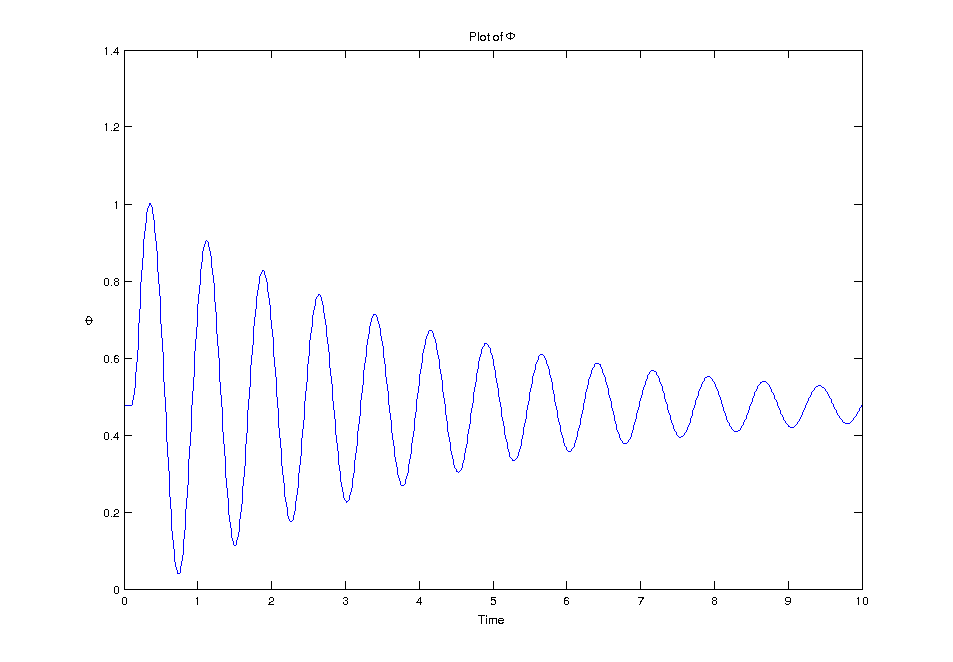
\includegraphics[width=1.2\linewidth]{../Code/miniApps/power_grid/phi_matlab.png}
%\label{fig:plot_of_phi_matlab}
%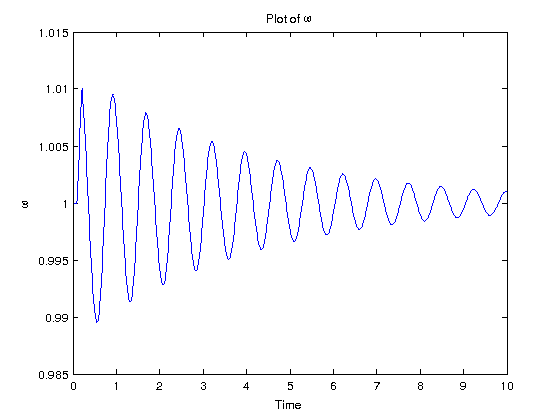
\includegraphics[width=1.2\linewidth]{../Code/miniApps/power_grid/omega_matlab.png}
%\label{fig:plot_of_omega_matlab}
%\end{figure}
\clearpage
\subsubsection{\texttt{Fortran} port}\label{sec_fortran_port_porous}
%The directory \texttt{Fortran/ContinousAdj} contains the port of the \texttt{MATLAB} version. L-BFGS \cite{Byrd_1996},\cite{Zhu_1997},\cite{Morales_2011} was used to perform the optimization in the \texttt{Fortran} port, a copy of which can be obtained \href{http://users.iems.northwestern.edu/~nocedal/lbfgsb.html}{here}.\\
%
%\noindent The directory \texttt{Fortran/ContinousAdj} contains the files to compile continous adjoint version of the optimal control problem listed in \ref{power_cont_adj_math} and \cite{Rao_2013}. The binaries (\textbf{files}), corresponding to these, on building the directory are \texttt{powergrid} (\textbf{{main.f90}}).\\
%
%\noindent The listing of files and their descriptions follow.\\
%
%\dirtree{%
%.1 /. 
%.2 Fortran/ContinuousAdj.  
%.3 blas.f\DTcomment{L-BFGS support file}. 
%.3 constants.f90\DTcomment{Constants and shared variables}. 
%.3 gnufor2.f90\DTcomment{\texttt{Fortran} bindings for GNUPlot}. 
%.3 iterate.dat\DTcomment{Output from L-BFGS optimization routine}. 
%.3 lbfgsb.f\DTcomment{L-BFGS optimization routine}. 
%.3 linpack.f\DTcomment{L-BFGS support file}. 
%.3 main.f90\DTcomment{Driver for the continuous adjoint port}. 
%.3 Makefile\DTcomment{Build commands}. 
%.3 print\_active.f\DTcomment{Routines to pretty print matrices and vectors}. 
%.3 timer.f\DTcomment{L-BFGS support file}. 
%}
%\hfill \break
%\noindent The plots generated by the \texttt{Fortran} version using continuous adjoints appear on the following page.
%\clearpage
%\begin{figure}[h]
%\centering
%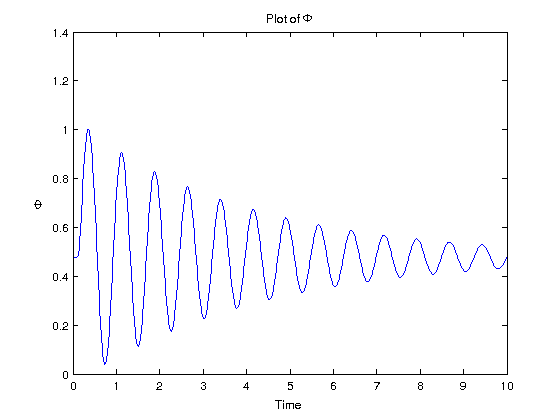
\includegraphics[width=1.2\linewidth]{../Code/miniApps/power_grid/phi_fortran_ca.png}
%\label{fig:plot_of_phi_fortran_ca}
%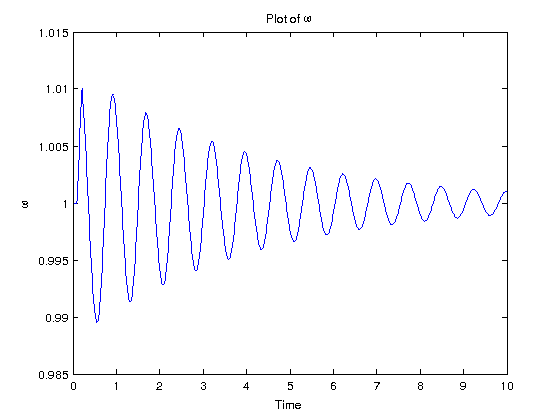
\includegraphics[width=1.2\linewidth]{../Code/miniApps/power_grid/omega_fortran_ca.png}
%\label{fig:plot_of_omega_fortran_ca}
%\end{figure}
%\clearpage
\subsubsection{\texttt{Fortran} port with \texttt{OpenAD/F} in Reverse Joint Mode}
%For details on reverse split mode refer \cite{Griewank_2008} and \cite{Utke_2014}.\\
%
%\noindent The directory \texttt{Fortran/DiscreteAdj/OpenAD/Split} contains the files to compile the discrete adjoint version of the \texttt{Fortran} port in section \ref{sec_fortran_port_power}. L-BFGS \cite{Byrd_1996},\cite{Zhu_1997},\cite{Morales_2011} was used to perform the optimization in the discrete adjoint version of the Fortran port, a copy of which can be obtained \href{http://users.iems.northwestern.edu/~nocedal/lbfgsb.html}{here}.\\
%
%\noindent The binaries (\textbf{files}), corresponding to these, on building the directory are \texttt{powergrid} (\textbf{{main.f90}}).\\
%
%\noindent The adjoint version of the forward model is used in the file  \texttt{main.f90}. These have been obtained by passing the undifferentiated routines to \texttt{OpenAD/F} in reverse-split mode.\\
%
%\noindent For details on how to call \texttt{OpenAD/F} in reverse-split mode refer \cite{Utke_2014}. The listing of files and their descriptions follow.\\
%
%\dirtree{%
%.1 /. 
%.2 Fortran/DiscreteAdj/OpenAD/Split.  
%.3 blas.f\DTcomment{L-BFGS support file}. 
%.3 constants.f90\DTcomment{Constants and shared variables}. 
%.3 gnufor2.f90\DTcomment{\texttt{Fortran} bindings for GNUPlot}. 
%.3 iterate.dat\DTcomment{Output from L-BFGS optimization routine}. 
%.3 lbfgsb.f\DTcomment{L-BFGS optimization routine}. 
%.3 linpack.f\DTcomment{L-BFGS support file}. 
%.3 main.f90\DTcomment{Driver for the discrete adjoint of port}. 
%.3 Makefile\DTcomment{Build commands}. 
%.3 Makefile\_continuous\_adjoint\DTcomment{Build commands for CA model}. 
%.3 numerics.f90\DTcomment{FW and CA model routines from \texttt{main.f90}}. 
%.3 print\_active.f\DTcomment{Routines to pretty print matrices and vectors}. 
%.3 timer.f\DTcomment{L-BFGS support file}.  
%}
%
%\hfill \break
%\noindent The plots generated by the \texttt{Fortran} version using discrete adjoints generated by \texttt{OpenAD/F} in reverse-split mode appear on the following page.
%
%\clearpage
%\begin{figure}[h]
%\centering
%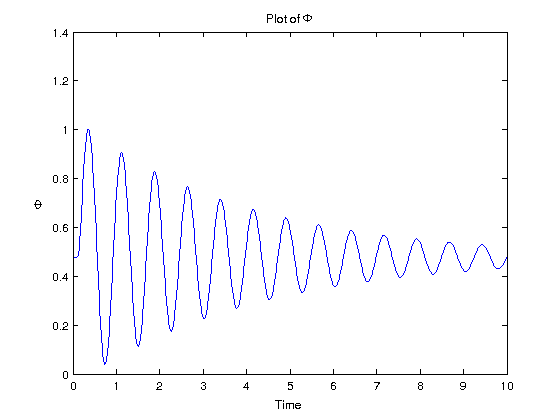
\includegraphics[width=1.2\linewidth]{../Code/miniApps/power_grid/phi_fortran_da_oad_rs.png}
%\label{fig:phi_fortran_da_oad_rs}
%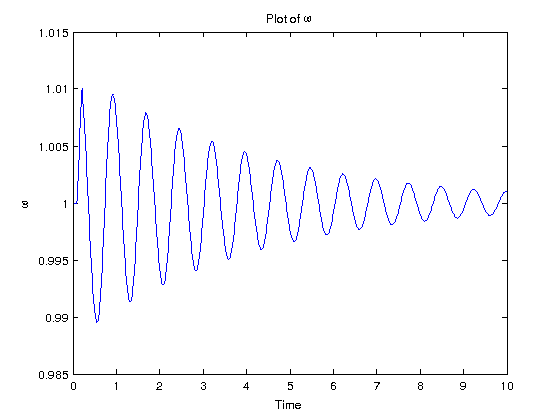
\includegraphics[width=1.2\linewidth]{../Code/miniApps/power_grid/omega_fortran_da_oad_rs.png}
%\label{fig:omega_fortran_da_oad_rs}
%\end{figure}
%\clearpage
%\subsection{Modifications performed}
\subsection{How to build}
%Running make as below, in each of the five subdirectories beginning with \texttt{Fortran/} will build the  binary \texttt{powergrid}
%\hfill\break
%\begin{lstlisting}[language=mybash, numbers=none]
%    $ make
%\end{lstlisting}
\subsection{How to verify}
%At the time of writing, there exists no script that can validate the output from any of the binaries. All versions of the binary \texttt{powergrid} should produce similar (in some sense/nearby) optimal and objective values.\\
%
%\noindent Validation by eyeballing the output from each version of the binary  \texttt{powergrid} has been performed. 
%
%\begin{TodoPar}
%\noindent It will be valuable to write a \texttt{python} script that will take as input two \texttt{csv} files and find the \texttt{max-norm} of the difference between the corresponding entries. Other norms may also be computed. 
%\end{TodoPar}
%
%\begin{HypoPar}
%\noindent I wonder it might be difficult to test the derivatives of each version of \texttt{powergrid} against another, since the code does not do computations deterministically i.e. there are convergence related iterations, each version may take different trajectories (except at the starting point) until they arrive at nearby solutions that are similar as metioned earlier.\\
%
%\noindent One solution, might be to generate multiple experiments with several different starting points and compare the derivatives at the starting points alone.
%\end{HypoPar}


%\subsection{How to extend}
 \clearpage

\section{Appendix}
\subsection{AirFoil}\label{diff_airfoil}
\subsubsection{diff of air\_foil\_tapenade and the original source}
\lstinputlisting[language=mydiff]{../Code/miniApps/airfoil/airfoil_tapenade.diff}

\newpage
\bibliographystyle{acm}
\bibliography{report}  

\newpage
\vfill
\begin{flushright}
\scriptsize
\framebox{\parbox{2.4in}{The submitted manuscript has been created by
UChicago Argonne, LLC, Operator of Argonne National Laboratory
(``Argonne").  Argonne, a U.S. Department of Energy Office
of Science laboratory, is operated under Contract No.
DE-AC02-06CH11357.  The U.S. Government retains for itself, and
others acting on its behalf, a paid-up, nonexclusive, irrevocable
worldwide license in said article to reproduce, prepare derivative works,
distribute copies to the public, and perform publicly and display
publicly, by or on behalf of the Government.}}
\normalsize
\end{flushright}

% that's all folks
\end{document}


